% !TeX program = xelatex
\documentclass[a4paper,10pt]{article}

% ============================================================================
% កញ្ចប់បណ្ណាល័យ (Packages) – តាមលំនាំស្តង់ដារ អនុវិទ្យាល័យព្រះក្រសាំង (ls_plan.tex)
% បរិបទ៖ ថ្នាក់រៀនគ្មានស្លាយ LCD – បង្រៀនដោយប្រើក្ដារខៀន រ៉ាប់ព័រទ័រ ដែកឈាន និងសន្លឹកកិច្ចការស-ខ្មៅ
% ============================================================================
\usepackage[a4paper, left=0.95cm, right=0.95cm, top=0.85cm, bottom=0.92cm, footskip=0.52cm]{geometry}
\usepackage{amsmath}
\usepackage{unicode-math}
\usepackage{fontspec}
\usepackage{array, longtable, multirow, colortbl}
\usepackage[table]{xcolor}
\usepackage{enumitem}
\usepackage{pifont}
\usepackage{fancyhdr}
\usepackage{tikz}
\usetikzlibrary{calc, arrows.meta, angles, quotes, decorations.markings, positioning, babel}

\makeatletter
\let\@expl@@@mark@update@singlecol@structures@@\relax
\makeatother

% ============================================================================
% ការកំណត់ពុម្ពអក្សរផ្លូវការ (Cross-Platform Fonts Configuration)
% ============================================================================
\providecommand{\NGSFindFonts}{%
  \IfFileExists{C:/Windows/Fonts/cambria.ttc}{%
    \def\NGSSysPath{C:/Windows/Fonts/}%
    \def\NGSUserPath{C:/Users/KIT/AppData/Local/Microsoft/Windows/Fonts/}%
  }{%
    \IfFileExists{./fonts/KhmerOSsiemreap.ttf}{\def\NGSSysPath{./fonts/}\def\NGSUserPath{./fonts/}}{%
    \IfFileExists{../fonts/KhmerOSsiemreap.ttf}{\def\NGSSysPath{../fonts/}\def\NGSUserPath{../fonts/}}{%
    \IfFileExists{../../fonts/KhmerOSsiemreap.ttf}{\def\NGSSysPath{../../fonts/}\def\NGSUserPath{../../fonts/}}{%
    \IfFileExists{../../../fonts/KhmerOSsiemreap.ttf}{\def\NGSSysPath{../../../fonts/}\def\NGSUserPath{../../../fonts/}}{%
    \IfFileExists{../../../../fonts/KhmerOSsiemreap.ttf}{\def\NGSSysPath{../../../../fonts/}\def\NGSUserPath{../../../../fonts/}}{%
    \IfFileExists{../../../../../fonts/KhmerOSsiemreap.ttf}{\def\NGSSysPath{../../../../../fonts/}\def\NGSUserPath{../../../../../fonts/}}{%
    \IfFileExists{../../../../../../fonts/KhmerOSsiemreap.ttf}{\def\NGSSysPath{../../../../../../fonts/}\def\NGSUserPath{../../../../../../fonts/}}{%
      \def\NGSSysPath{../../../../../../../fonts/}\def\NGSUserPath{../../../../../../../fonts/}%
    }}}}}}}%
  }%
}
\NGSFindFonts

\setmathfont[Path={\NGSSysPath}, FontIndex=1, Scale=1.02]{cambria.ttc}
\defaultfontfeatures{Ligatures=TeX}

\setmainfont[
  Path={\NGSUserPath},
  Extension=.ttf,
  Script=Khmer,
  BoldFont={KhmerOSsiemreap},
  BoldFeatures={FakeBold=1.8},
  ItalicFont={KhmerOSsiemreap},
  ItalicFeatures={FakeSlant=0.25},
  BoldItalicFont={KhmerOSsiemreap},
  BoldItalicFeatures={FakeBold=1.8, FakeSlant=0.25}
]{KhmerOSsiemreap}

\newfontfamily\muol[Path={\NGSUserPath}, Extension=.ttf, Script=Khmer]{KhmerOSmuollight}
\newfontfamily\TimesEn[Path={\NGSSysPath}, Extension=.ttf, BoldFont={timesbd}, ItalicFont={timesi}, BoldItalicFont={timesbi}]{times}
\newfontfamily\NagaBold[Path={\NGSUserPath}, Extension=.ttf]{AKbalthom Naga Bold}
\newfontfamily\CalibriFont[Path={\NGSSysPath}, Extension=.ttf]{calibri}
\newfontfamily\Tacteing[Path={\NGSUserPath}]{TACTENG.TTF}
\newfontfamily\CourierBullet[Path={\NGSSysPath}, Extension=.ttf]{cour}
\newcommand{\wcirc}{{\CourierBullet\fontsize{9.5pt}{11pt}\selectfont o}}

\XeTeXlinebreaklocale "km"
\XeTeXlinebreakskip = 0pt plus 1pt minus 0.1pt

\definecolor{stepgray}{HTML}{D9D9D9}
\definecolor{headgray}{HTML}{F2F2F2}
\definecolor{boxgray}{HTML}{D9D9D9}
\definecolor{darkred}{HTML}{C00000}
\definecolor{red5e}{HTML}{FF0000}

\pagestyle{fancy}
\fancyhf{}
\renewcommand{\headrulewidth}{0pt}
\fancyfoot[R]{\CalibriFont\fontsize{11pt}{13pt}\selectfont\thepage}

\setlength{\parindent}{0pt}
\setlength{\parskip}{0pt}
\setlength{\tabcolsep}{3.8pt}

\newcolumntype{L}[1]{>{\raggedright\arraybackslash}p{#1}}

\newcommand{\en}[1]{{\TimesEn #1}}
\newcommand{\enbf}[1]{{\TimesEn\textbf{#1}}}
\newcommand{\unit}[1]{\,\text{\en{#1}}}
\newcommand{\fiveE}[1]{{\NagaBold\fontsize{9.5pt}{13pt}\selectfont\textcolor{red5e}{#1}}}
\newcommand{\timenote}[1]{\textcolor{darkred}{\textit{#1}}}
\newcommand{\graybox}[1]{\colorbox{boxgray}{\strut\hspace{2pt}#1\hspace{2pt}}}
\newcommand{\ditem}{\tikz[baseline=-0.5ex]\fill (0,0.42ex) -- (0.42ex,0) -- (0,-0.42ex) -- (-0.42ex,0) -- cycle;\hspace{0.3em}}
\newcommand{\cnum}[1]{{\fontsize{10.5pt}{12pt}\selectfont\ding{\numexpr171+#1\relax}}\hspace{0.2em}}
\newcommand{\cfig}[1]{\par\vspace{4pt}{\centering #1\par}\vspace{4pt}}
\newcommand{\stepheader}[1]{\multicolumn{3}{|c|}{\cellcolor{stepgray}\muol #1} \\* \noalign{\hrule height 0.4pt}}
\newcommand{\tri}[1]{\ensuremath{\triangle #1}}
\newcommand{\ang}[1]{\ensuremath{\angle #1}}
\newcommand{\arc}[1]{\ensuremath{\widehat{#1}}}
\newcommand{\cg}{\ensuremath{\cong}}
\newcommand{\khmflourish}{{\Tacteing\fontsize{36pt}{14pt}\selectfont\raisebox{-5pt}{3}}}

\tikzset{
  tk1/.style={postaction={decorate},decoration={markings,mark=at position 0.50 with {\draw[black, line width=0.85pt](0,-0.095)--(0,0.095);}}},
  tk2/.style={postaction={decorate},decoration={markings,
    mark=at position 0.45 with {\draw[black, line width=0.85pt](0,-0.095)--(0,0.095);},
    mark=at position 0.55 with {\draw[black, line width=0.85pt](0,-0.095)--(0,0.095);}}}
}

% ============================================================================
% ម៉ាក្រូរូបភាពធរណីមាត្រស-ខ្មៅ (Proportional 4.2–7.2 cm B&W TikZ Diagrams)
% ============================================================================

% ១. កំណែកិច្ចការផ្ទះទី៧ (ទំ.២០៤) + E1 Engage ផ្លូវរត់កោងរួមផ្ចិតពីរគន្លង (r1=10m, r2=20m)
\newcommand{\figEngageCIRCTwo}{%
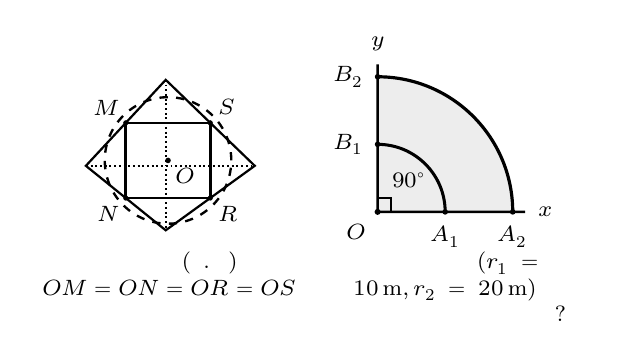
\begin{tikzpicture}[scale=0.78, every node/.style={font=\footnotesize, text=black}]
  % ឆ្វេង៖ កំណែលំហាត់ទី៧ ទំ.២០៤ (MNRS ចតុកោណកែង => លើរង្វង់ផ្ចិត O)
  \begin{scope}[shift={(0,0)}]
    \coordinate (A) at (1.50,2.55);
    \coordinate (B) at (0.20,1.15);
    \coordinate (C) at (1.50,0.10);
    \coordinate (D) at (2.95,1.15);
    \coordinate (M) at ($(A)!0.5!(B)$);
    \coordinate (N) at ($(B)!0.5!(C)$);
    \coordinate (R) at ($(C)!0.5!(D)$);
    \coordinate (S) at ($(D)!0.5!(A)$);
    \coordinate (O) at ($(M)!0.5!(R)$);
    \draw[black, line width=0.80pt] (A)--(B)--(C)--(D)--cycle;
    \draw[black, line width=0.70pt, densely dotted] (A)--(C) (B)--(D);
    \draw[black, line width=0.95pt] (M)--(N)--(R)--(S)--cycle;
    \draw[black, line width=0.85pt, dashed] (O) circle (1.03);
    \fill[black] (O) circle (1.3pt) node[below right=-1pt] {$O$};
    \fill[black] (M) circle (1.2pt) node[above left=-1pt] {$M$};
    \fill[black] (N) circle (1.2pt) node[below left=-1pt] {$N$};
    \fill[black] (R) circle (1.2pt) node[below right=-1pt] {$R$};
    \fill[black] (S) circle (1.2pt) node[above right=-1pt] {$S$};
    \node[anchor=north, text width=3.35cm, align=center] at (1.55,-0.10) {កំណែលំហាត់ទី៧ (ទំ.២០៤)៖\\$OM=ON=OR=OS$};
  \end{scope}
  % ស្ដាំ៖ បេសកកម្ម E1 ផ្លូវរត់កោងរួមផ្ចិត O មុំ 90° (r1=10m vs r2=20m)
  \begin{scope}[shift={(4.50,0.15)}]
    \coordinate (O) at (0.45,0.25);
    \fill[gray!14] (O) -- ++(0:2.20) arc (0:90:2.20) -- cycle;
    \draw[black, line width=0.95pt] (O) -- (2.85,0.25) node[right=1pt] {$x$};
    \draw[black, line width=0.95pt] (O) -- (0.45,2.65) node[above=1pt] {$y$};
    \draw[black, line width=1.10pt] ($(O)+(0:1.10)$) arc (0:90:1.10);
    \draw[black, line width=1.15pt] ($(O)+(0:2.20)$) arc (0:90:2.20);
    \draw[black, line width=0.70pt] (O) rectangle ++(0.22,0.22);
    \fill[black] (O) circle (1.4pt) node[below left=1pt] {$O$};
    \fill[black] ($(O)+(0:1.10)$) circle (1.3pt) node[below=1.5pt] {$A_1$};
    \fill[black] ($(O)+(90:1.10)$) circle (1.3pt) node[left=1.5pt] {$B_1$};
    \fill[black] ($(O)+(0:2.20)$) circle (1.3pt) node[below=1.5pt] {$A_2$};
    \fill[black] ($(O)+(90:2.20)$) circle (1.3pt) node[left=1.5pt] {$B_2$};
    \node at ($(O)+(45:0.72)$) {$90^\circ$};
    \node[anchor=north, text width=3.55cm, align=center] at (1.55,-0.25) {ផ្លូវរត់កោងរួមផ្ចិត ($r_1=10\unit{m}, r_2=20\unit{m}$)\\តើដឺក្រេធ្នូ និងប្រវែងធ្នូស្មើគ្នាឬទេ?};
  \end{scope}
\end{tikzpicture}}

% ២. E2 & E3: មុំផ្ចិតលយ/ឆក និងកាដ្រង់ (ទំ.១៩៩) + ធ្នូប៉ុនគ្នាស្កាត់ដោយមុំផ្ចិតប៉ុនគ្នា
\newcommand{\figCentralAnglesCIRCTwo}{%
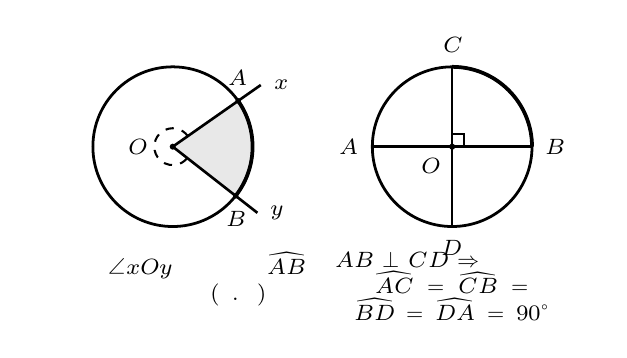
\begin{tikzpicture}[scale=0.78, every node/.style={font=\footnotesize, text=black}]
  % ឆ្វេង៖ ឧទាហរណ៍ទី១ (ទំ.១៩៩) មុំផ្ចិតលយ និងមុំផ្ចិតឆក xOy
  \begin{scope}[shift={(0,0)}]
    \coordinate (O) at (1.55,1.40);
    \fill[gray!18] (O) -- ($(O)+(35:1.30)$) arc (35:-38:1.30) -- cycle;
    \draw[black, line width=1.0pt] (O) circle (1.30);
    \draw[black, line width=0.95pt] (O) -- ($(O)+(35:1.75)$) node[right=1pt] {$x$};
    \draw[black, line width=0.95pt] (O) -- ($(O)+(-38:1.75)$) node[right=1pt] {$y$};
    \draw[black, line width=1.35pt] ($(O)+(35:1.30)$) arc (35:-38:1.30);
    \draw[black, line width=0.75pt, dashed] ($(O)+(35:0.30)$) arc (35:322:0.30);
    \fill[black] (O) circle (1.4pt);
    \node[left=5.5pt] at (O) {$O$};
    \fill[black] ($(O)+(35:1.30)$) circle (1.3pt) node[above=2pt] {$A$};
    \fill[black] ($(O)+(-38:1.30)$) circle (1.3pt) node[below=2pt] {$B$};
    \node[anchor=north, text width=3.45cm, align=center] at (1.55,-0.15) {មុំផ្ចិតលយ $\ang{xOy}$ ស្កាត់ធ្នូតូច $\arc{AB}$\\និងមុំឆកស្កាត់ធ្នូធំ (ទំ.១៩៩)};
  \end{scope}
  % ស្ដាំ៖ ឧទាហរណ៍ទី២ និងទី៣ (ធ្នូប៉ុនគ្នា និងកាដ្រង់ 90°)
  \begin{scope}[shift={(4.50,0)}]
    \coordinate (O) at (1.60,1.40);
    \draw[black, line width=1.0pt] (O) circle (1.30);
    \draw[black, line width=0.90pt] ($(O)+(180:1.30)$) -- ($(O)+(0:1.30)$);
    \draw[black, line width=0.90pt] ($(O)+(270:1.30)$) -- ($(O)+(90:1.30)$);
    \draw[black, line width=0.70pt] (O) rectangle ++(0.20,0.20);
    \draw[black, line width=1.35pt] ($(O)+(0:1.30)$) arc (0:90:1.30);
    \fill[black] (O) circle (1.4pt) node[below left=1pt] {$O$};
    \node[left=1.5pt] at ($(O)+(180:1.30)$) {$A$};
    \node[right=1.5pt] at ($(O)+(0:1.30)$) {$B$};
    \node[above=1.5pt] at ($(O)+(90:1.30)$) {$C$};
    \node[below=1.5pt] at ($(O)+(270:1.30)$) {$D$};
    \node[above right=1pt] at ($(O)+(45:1.30)$) {កាដ្រង់};
    \node[anchor=north, text width=3.50cm, align=center] at (1.60,-0.15) {$AB \perp CD \Rightarrow$ កាដ្រង់ទាំង ៤\\$\arc{AC}=\arc{CB}=\arc{BD}=\arc{DA}=90^\circ$};
  \end{scope}
\end{tikzpicture}}

% ៣. E4 & E5: លំហាត់គំរូទី១-២ (ប្រវែងធ្នូ ទំ.២០០) + ប្រតិបត្តិ ទំ.២០០ (ធ្នូ AB < ធ្នូ CD)
\newcommand{\figArcLengthPractCIRCTwo}{%
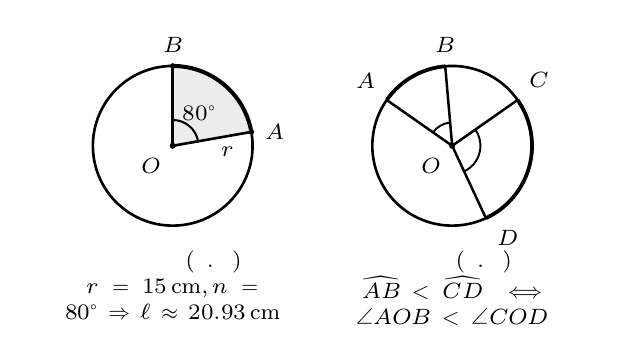
\begin{tikzpicture}[scale=0.78, every node/.style={font=\footnotesize, text=black}]
  % ឆ្វេង៖ លំហាត់គំរូទី២ ទំ.២០០ (r = 15 cm, មុំផ្ចិត 80°)
  \begin{scope}[shift={(0,0)}]
    \coordinate (O) at (1.55,1.40);
    \fill[gray!14] (O) -- ($(O)+(10:1.30)$) arc (10:90:1.30) -- cycle;
    \draw[black, line width=0.95pt] (O) circle (1.30);
    \draw[black, line width=0.95pt] (O) -- ($(O)+(10:1.30)$);
    \draw[black, line width=0.95pt] (O) -- ($(O)+(90:1.30)$);
    \draw[black, line width=1.45pt] ($(O)+(10:1.30)$) arc (10:90:1.30);
    \draw[black, line width=0.75pt] ($(O)+(10:0.42)$) arc (10:90:0.42);
    \fill[black] (O) circle (1.4pt) node[below left=1pt] {$O$};
    \fill[black] ($(O)+(10:1.30)$) circle (1.3pt) node[right=1.5pt] {$A$};
    \fill[black] ($(O)+(90:1.30)$) circle (1.3pt) node[above=1.5pt] {$B$};
    \node at ($(O)+(50:0.68)$) {$80^\circ$};
    \node[below right=-1pt] at ($(O)+(10:0.68)$) {$r$};
    \node[anchor=north, text width=3.45cm, align=center] at (1.55,-0.15) {លំហាត់គំរូទី២ (ទំ.២០០)៖\\$r=15\unit{cm}, n=80^\circ \Rightarrow \ell\approx 20.93\unit{cm}$};
  \end{scope}
  % ស្ដាំ៖ ប្រតិបត្តិ ទំ.២០០ (ធ្នូ AB < ធ្នូ CD => <AOB < <COD)
  \begin{scope}[shift={(4.50,0)}]
    \coordinate (O) at (1.60,1.40);
    \draw[black, line width=0.95pt] (O) circle (1.30);
    \coordinate (A) at ($(O)+(145:1.30)$);
    \coordinate (B) at ($(O)+(95:1.30)$);
    \coordinate (C) at ($(O)+(35:1.30)$);
    \coordinate (D) at ($(O)+(-65:1.30)$);
    \draw[black, line width=0.90pt] (A)--(O)--(B) (C)--(O)--(D);
    \draw[black, line width=1.35pt] (B) arc (95:145:1.30);
    \draw[black, line width=1.35pt] (D) arc (-65:35:1.30);
    \draw[black, line width=0.70pt] ($(O)+(95:0.38)$) arc (95:145:0.38);
    \draw[black, line width=0.70pt] ($(O)+(-65:0.46)$) arc (-65:35:0.46);
    \fill[black] (O) circle (1.4pt) node[below left=1pt] {$O$};
    \node[above left=1pt] at (A) {$A$};
    \node[above=1.5pt] at (B) {$B$};
    \node[above right=1pt] at (C) {$C$};
    \node[below right=1pt] at (D) {$D$};
    \node[anchor=north, text width=3.50cm, align=center] at (1.60,-0.15) {ប្រតិបត្តិ (ទំ.២០០)៖\\$\arc{AB} < \arc{CD} \iff \ang{AOB} < \ang{COD}$};
  \end{scope}
\end{tikzpicture}}

\begin{document}
\fontsize{10pt}{15.2pt}\selectfont

% -------------------- ក្បាលកិច្ចតែងការ (Header) --------------------
\begin{center}
  {\muol\fontsize{11pt}{16pt}\selectfont ព្រះរាជាណាចក្រកម្ពុជា}\\[2pt]
  {\muol\fontsize{10pt}{15pt}\selectfont ជាតិ សាសនា ព្រះមហាក្សត្រ}\\[1pt]
  \khmflourish
\end{center}

\vspace{-28pt}
{\muol\fontsize{9.5pt}{12.5pt}\selectfont
មន្ទីរអប់រំ យុវជន និងកីឡា ខេត្តកំពង់ធំ\\
ការិយាល័យអប់រំ យុវជន និងកីឡា ស្រុកកំពង់ស្វាយ\\
អនុវិទ្យាល័យព្រះក្រសាំង}

\vspace{1pt}
\begin{center}
  {\muol\fontsize{10pt}{14pt}\selectfont កិច្ចតែងការបង្រៀន}
\end{center}
\vspace{0pt}

% -------------------- ព័ត៌មានទូទៅ (Metadata) --------------------
{\renewcommand{\arraystretch}{0.95}
\hspace*{4.05cm}%
\begin{tabular}{@{}l l l@{}}
  - \hspace{0.35cm} មុខវិជ្ជា & : & គណិតវិទ្យា ថ្នាក់ទី៨ \\
  - \hspace{0.35cm} ចំណងជើងមេរៀន & : & មេរៀនទី១៥ រង្វង់ \\
  - \hspace{0.35cm} ចំណងជើងរង & : & ២. មុំផ្ចិត និងធ្នូ (សៀវភៅសិក្សាគោល ទំ.១៩៩--២០០ និងទំ.២០៤) \\
  - \hspace{0.35cm} រយៈពេល & : & ១ ម៉ោងសិក្សា (៥០ នាទី) \\
  - \hspace{0.35cm} បង្រៀនដោយ & : & ហុក ប៊ុនថែន \\
  - \hspace{0.35cm} កាលបរិច្ឆេទ & : & ថ្ងៃសុក្រ ១រោច ខែមិគសិរ ព.ស.២៥៧០ (២៥ ធ្នូ ២០២៦) \\
\end{tabular}
}

\vspace{1pt}

% -------------------- I. វត្ថុបំណង --------------------
\textbf{I.} {\muol វត្ថុបំណង}\\[1pt]
\hspace*{0.55cm}%
\begin{tabular}{@{}l l L{14.2cm}@{}}
  \wcirc \hspace{0.25cm} វិជ្ជាសម្បទា & : & សិស្សពោលបានត្រឹមត្រូវនូវនិយមន័យមុំផ្ចិត (មុំលយ និងមុំឆក) ធ្នូស្កាត់ដោយមុំផ្ចិត កាដ្រង់ ($90^\circ$) លក្ខណៈសមមូលរវាងមុំផ្ចិត និងធ្នូស្កាត់ ($\ang{AOB}=\ang{DOE} \iff \arc{AB}=\arc{DE}$) ព្រមទាំងរូបមន្តប្រវែងធ្នូ $\ell = \dfrac{2\pi r \times n^\circ}{360^\circ}$ តាមសៀវភៅគោល ទំ.១៩៩--២០០ ។ \\
  \wcirc \hspace{0.25cm} បំណិនសម្បទា & : & សិស្សញែកដាច់រវាង \textbf{រង្វាស់គិតជាដឺក្រេនៃធ្នូ} ($n^\circ$) និង \textbf{ប្រវែងធ្នូគិតជាឯកតាប្រវែង} ($\ell$) គណនាប្រវែងធ្នូ ឬកាំ ឬមុំផ្ចិតដោយប្រើផលធៀបប្រភាគនៃបរិមាត្ររង្វង់ និងប្រៀបធៀបធ្នូពីរមិនប៉ុនគ្នាតាមមុំផ្ចិតលើសន្លឹកកិច្ចការស-ខ្មៅបានត្រឹមត្រូវ ។ \\
  \wcirc \hspace{0.25cm} ចរិយាសម្បទា & : & សិស្សមានទម្លាប់ពិនិត្យឯកតា ($^\circ$ ទល់នឹង $\text{\en{cm}}, \text{\en{dm}}, \text{\en{m}}$) មុនសន្និដ្ឋាន មិនច្រឡំថាធ្នូមានដឺក្រេស្មើគ្នាលើរង្វង់កាំខុសគ្នាត្រូវមានប្រវែងស្មើគ្នា និងឃើញតម្លៃអនុវត្តក្នុងការវាស់ផ្លូវកោង កង់រទេះ និងទ្រនិចនាឡិកា ។ \\
\end{tabular}

\vspace{1pt}

% -------------------- II. សម្ភារៈឧបទេស --------------------
\textbf{II.} {\muol សម្ភារៈឧបទេស}\\[1pt]
\hspace*{0.55cm}$\bullet$ \hspace{0.35cm} សៀវភៅសិក្សាគោលគណិតវិទ្យាថ្នាក់ទី៨ (ទំ.១៩៩--២០០ និងទំ.២០៤) ក្ដារខៀន ដីស បន្ទាត់ក្រិត រ៉ាប់ព័រទ័រ ដែកឈាន និងសន្លឹកកិច្ចការសិស្សស-ខ្មៅ (\en{Worksheet\_CIRC2} ចំនួន ២ ទំព័រ \en{A4} ដោយគ្មានស្លាយ \en{LCD}) ។

\vspace{1pt}

% -------------------- III. វិធីសាស្រ្តបង្រៀន --------------------
\textbf{III.} {\muol វិធីសាស្រ្តបង្រៀន}\\[1pt]
\hspace*{0.55cm}$\bullet$ \hspace{0.35cm} គោលវិធីសិស្សមជ្ឈមណ្ឌលតាមគំរូ \en{5Es} រួមបញ្ចូល \textbf{វិធីប្រៀបធៀបរង្វង់រួមផ្ចិត} (\en{Concentric Contrasting-Cases}, \en{Sidney et al., 2015}) និង \textbf{វិចារណញ្ញាណប្រភាគនៃបរិមាត្រ} (\en{Multiplicative-Fraction Arc Reasoning}, \en{Moore, 2013}) លើសន្លឹកកិច្ចការស-ខ្មៅ ។

\vspace{2pt}

% -------------------- IV. ដំណើរការបង្រៀន --------------------
\textbf{IV.} {\muol ដំណើរការបង្រៀន}\\[-6pt]

{\renewcommand{\arraystretch}{1.15}
\begin{longtable}{|L{5.50cm}|L{7.90cm}|L{4.80cm}|}
\hline
\multicolumn{1}{|c|}{\cellcolor{headgray}\muol សកម្មភាពគ្រូ} &
\multicolumn{1}{c|}{\cellcolor{headgray}\muol ខ្លឹមសារមេរៀន} &
\multicolumn{1}{c|}{\cellcolor{headgray}\muol សកម្មភាពសិស្ស} \\[2pt]
\hline
\endfirsthead

\hline
\multicolumn{1}{|c|}{\cellcolor{headgray}\muol សកម្មភាពគ្រូ} &
\multicolumn{1}{c|}{\cellcolor{headgray}\muol ខ្លឹមសារមេរៀន} &
\multicolumn{1}{c|}{\cellcolor{headgray}\muol សកម្មភាពសិស្ស} \\[2pt]
\hline
\endhead

\hline
\endfoot

% ==================== ជំហានទី១ (2min) ====================
\stepheader{ជំហានទី១ ៖ រដ្ឋបាលថ្នាក់ (២ នាទី)}
$\bullet$ ពិនិត្យអវត្តមាន សណ្ដាប់ធ្នាប់ អនាម័យ និងការត្រៀមរ៉ាប់ព័រទ័រ-បន្ទាត់ក្រិត \par\vspace{1pt}
$\bullet$ ចែកសន្លឹកកិច្ចការស-ខ្មៅ \en{Worksheet\_CIRC2} (១ សន្លឹកសងខាងក្នុងម្នាក់)
&
$\bullet$ វត្តមានសិស្ស វិន័យ និងការត្រៀមរ៉ាប់ព័រទ័រសម្រាប់វាស់មុំផ្ចិត \par\vspace{1pt}
$\bullet$ សន្លឹកកិច្ចការសិស្ស \en{Worksheet\_CIRC2} (មេរៀនទី១៥ ៖ ២. មុំផ្ចិត និងធ្នូ)
&
$\circ$ ប្រធានថ្នាក់រាយការណ៍អវត្តមាន \par\vspace{1pt}
$\circ$ ទទួលសន្លឹកកិច្ចការ សរសេរឈ្មោះ និងដាក់រ៉ាប់ព័រទ័រលើតុ \\
\hline

% ==================== ជំហានទី២ (9min) ====================
\stepheader{ជំហានទី២ ៖ កែកិច្ចការផ្ទះ រំលឹកមេរៀនចាស់ និងភ្ជាប់បញ្ហាថ្មី (៩ នាទី)}
\timenote{(កែកិច្ចការផ្ទះ $\le 3\unit{min}$)} \par
$\bullet$ ហៅសិស្ស ១ នាក់ឡើងសរសេរគន្លឹះសម្រាយបញ្ជាក់លំហាត់ទី៧ (ទំ.២០៤) លើក្ដារខៀន
&
\textbf{កំណែកិច្ចការផ្ទះ (លំហាត់ទី៧ ទំ.២០៤)៖} \par
$\bullet$ តាមទ្រឹស្ដីបទបាតមធ្យមត្រីកោណ៖ $MN \parallel AC \parallel SR$ និង $MS \parallel BD \parallel NR$ ហើយដោយ $AC \perp BD \Rightarrow MN \perp MS \Rightarrow MNRS$ ជា \textbf{ចតុកោណកែង} ។ \par
$\bullet$ យក $O$ ជាប្រសព្វអង្កត់ទ្រូង $MR$ និង $NS \Rightarrow OM = ON = OR = OS \Rightarrow M, N, R, S$ ស្ថិតនៅលើរង្វង់តែមួយផ្ចិត $O$ ។
&
$\circ$ ផ្ទៀងផ្ទាត់ចម្លើយក្នុងសៀវភៅលំហាត់ និងកែលម្អចំណុចខ្វះខាត \\[3pt]

\timenote{(រំលឹកមេរៀនទាក់ទង $3\unit{min}$)} \par
$\bullet$ សួររំលឹករូបមន្តបរិមាត្ររង្វង់ $P$ (ថ្នាក់ទី៧) និងរង្វាស់មុំជុំវិញចំណុចមួយពេញមួយជុំ
&
\textbf{រំលឹកចំណេះដឹងមូលដ្ឋានភ្ជាប់មេរៀនថ្មី៖} \par
១. បរិមាត្ររង្វង់កាំ $r$៖ $P = 2\pi r = \pi d$ (ដែល $\pi \approx 3.14$) ។ \par
២. រង្វាស់មុំពេញមួយជុំជុំវិញផ្ចិត $O$ ស្មើនឹង $360^\circ$ (មុំរាប $= 180^\circ$, មុំកែង $= 90^\circ$) ។
&
$\circ$ ឆ្លើយរំលឹក៖ «$P = 2\pi r$ និងមុំពេញមួយជុំជុំវិញ $O$ ស្មើនឹង $360^\circ$» \\[3pt]

\fiveE{E1 - Engage} \timenote{(3 min)} \par
$\bullet$ លើកបញ្ហា \textbf{«ផ្លូវរត់កោងរួមផ្ចិតពីរគន្លង»} លើក្ដារខៀន និងផ្នែកទី១ នៃសន្លឹកកិច្ចការ \par
\hspace*{0.3em}– សំណួរ៖ «បើកីឡាករពីរនាក់រត់តាមគន្លងកោងមុំកែង $90^\circ$ ដូចគ្នា ($r_1=10\unit{m}$ និង $r_2=20\unit{m}$) តើពួកគេបត់បាន \textbf{ដឺក្រេធ្នូ} ស្មើគ្នា ឬ \textbf{ចម្ងាយម៉ែត្រ} ស្មើគ្នា?»
&
\textbf{បេសកកម្ម E1 ៖ ផ្លូវរត់កោងរួមផ្ចិតនៅទីលានកីឡា} \par
ទីលានរត់កោងរួមផ្ចិត $O$ មានគន្លងក្នុងកាំ $r_1 = 10\unit{m}$ (ធ្នូ $\arc{A_1B_1}$) និងគន្លងក្រៅកាំ $r_2 = 20\unit{m}$ (ធ្នូ $\arc{A_2B_2}$) ស្កាត់ដោយមុំកែង $\ang{xOy} = 90^\circ$ តែមួយ ។ \par
$\bullet$ \textbf{មតិទី១៖} មុំផ្ចិត $90^\circ$ ដូចគ្នា ដូច្នេះប្រវែងផ្លូវកោងទាំងពីរស្មើគ្នា ។ \par
$\bullet$ \textbf{មតិទី២៖} ដឺក្រេធ្នូស្មើគ្នា ($90^\circ$) តែប្រវែងគន្លងក្រៅវែងជាងគន្លងក្នុង $2$ ដង ។
&
$\circ$ អានបេសកកម្មលើសន្លឹកកិច្ចការ និងគូសធីកទស្សន៍ទាយមតិទី១ ឬមតិទី២ \\[3pt]

&
\cfig{\figEngageCIRCTwo}
& \\[3pt]
\hline

% ==================== ជំហានទី៣ (17min) ====================
\stepheader{ជំហានទី៣ ៖ មេរៀនថ្មី — មុំផ្ចិត និងធ្នូ (១៧ នាទី)}
\fiveE{E2 - Explore} \timenote{(11 min)} \par
\ditem \textbf{សកម្មភាពទី១៖ វាស់មុំផ្ចិត ធ្នូប៉ុនគ្នា និងកាដ្រង់ ($5\unit{min}$)} \par
$\bullet$ ឱ្យដៃគូសិស្សប្រើរ៉ាប់ព័រទ័រវាស់មុំផ្ចិតលើរង្វង់ខ្នាតពិត $1:1$ (ផ្នែកទី២ នៃសន្លឹកកិច្ចការ)៖ សម្គាល់មុំលយ $\ang{AOB}$ មុំឆក និងពិនិត្យពេលអង្កត់ផ្ចិតពីរកែងគ្នា ($AB \perp CD$)
&
\textbf{១. រុករកមុំផ្ចិត ធ្នូស្កាត់ និងកាដ្រង់ (ឧទាហរណ៍ទី១--៣ ទំ.១៩៩)៖} \par
$\bullet$ កន្លះបន្ទាត់ $Ox, Oy$ ចេញពីផ្ចិត $O$ បង្កើតបាន \textbf{មុំផ្ចិត} ពីរ៖ \textbf{មុំលយ} ($\le 180^\circ$) ស្កាត់ធ្នូតូច $\arc{AB}$ និង \textbf{មុំឆក} ($> 180^\circ$) ស្កាត់ធ្នូធំ ។ \par
$\bullet$ លើរង្វង់តែមួយ វាស់ឃើញ $\ang{AOB} = \ang{DOE} = 60^\circ \iff$ ធ្នូ $\arc{AB}$ និង $\arc{DE}$ មានប្រវែងត្រួតស៊ីគ្នាបេះបិទ ។ \par
$\bullet$ បើអង្កត់ផ្ចិត $AB \perp CD \Rightarrow$ មុំផ្ចិតទាំង ៤ ស្មើនឹង $90^\circ$ ចែករង្វង់ជា ៤ ធ្នូប៉ុនគ្នា ហៅថា \textbf{កាដ្រង់} ($\frac{1}{4}$ នៃរង្វង់) ។
&
$\circ$ ប្រើរ៉ាប់ព័រទ័រវាស់មុំផ្ចិតលើរូបខ្នាតពិត $1:1$ និងបំពេញឈ្មោះមុំលយ មុំឆក និងកាដ្រង់លើសន្លឹកកិច្ចការ \\[3pt]

\ditem \textbf{សកម្មភាពទី២៖ អន្ទាក់រង្វង់រួមផ្ចិតពីរ និងប្រភាគបរិមាត្រ ($6\unit{min}$)} \par
$\bullet$ ឱ្យសិស្សពិនិត្យរូបរង្វង់រួមផ្ចិតពីរខ្នាតពិត $1:1$ ($r_1 = 1\unit{cm}$ និង $r_2 = 2\unit{cm}$) ស្កាត់ដោយមុំកែង $90^\circ$ លើសន្លឹកកិច្ចការ៖ \par
\hspace*{0.3em}– ប្រៀបធៀបប្រភាគនៃរង្វង់ ($\frac{90^\circ}{360^\circ}$) និងគណនាប្រវែងធ្នូ $\ell_1, \ell_2$ រួចទាញរូបមន្តទូទៅសម្រាប់មុំផ្ចិត $n^\circ$
&
\textbf{២. បំបែកការយល់ច្រឡំ៖ រង្វាស់ដឺក្រេធ្នូ ($n^\circ$) ទល់នឹងប្រវែងធ្នូ ($\ell$)៖} \par
$\bullet$ ទាំងធ្នូក្នុង $\arc{A_1B_1}$ និងធ្នូក្រៅ $\arc{A_2B_2}$ សុទ្ធតែត្រូវនឹង $\dfrac{90^\circ}{360^\circ} = \dfrac{1}{4}$ នៃរង្វង់រៀងខ្លួន $\Rightarrow$ មាន \textbf{រង្វាស់ដឺក្រេស្មើគ្នាគឺ $90^\circ$} ។ \par
$\bullet$ ប៉ុន្តែ \textbf{ប្រវែងធ្នូគិតជា $\text{\en{cm}}$} មិនស្មើគ្នាទេ ($\pi \approx 3.14$)៖ \par
\hspace*{0.3em}– រង្វង់ក្នុង ($r_1=1\unit{cm}$)៖ $\ell_1 = \frac{1}{4}(2\pi r_1) = \frac{1}{4}(6.28) = \mathbf{1.57\unit{cm}}$ ។ \par
\hspace*{0.3em}– រង្វង់ក្រៅ ($r_2=2\unit{cm}$)៖ $\ell_2 = \frac{1}{4}(2\pi r_2) = \frac{1}{4}(12.56) = \mathbf{3.14\unit{cm}} = 2\ell_1$ ។ \par
$\bullet$ ជាទូទៅ បើមុំផ្ចិតស្មើនឹង $n^\circ$ ធ្នូស្មើនឹងប្រភាគ $\dfrac{n^\circ}{360^\circ}$ នៃបរិមាត្រ $P = 2\pi r$ ។
&
$\circ$ គណនាឃើញ $\ell_1=1.57\unit{cm} \ne \ell_2=3.14\unit{cm}$ បដិសេធមតិទី១ \par\vspace{1pt}
$\circ$ ទាញបានសមាមាត្រប្រភាគ $\ell = \dfrac{n^\circ}{360^\circ}\times 2\pi r$ \\[3pt]

&
\cfig{\figCentralAnglesCIRCTwo}
& \\[3pt]

\fiveE{E3 - Explain} \timenote{(6 min)} \par
$\bullet$ សំយោគនិយមន័យ លក្ខណៈទូទៅ និងសម្គាល់តាមសៀវភៅគោល ទំ.១៩៩ លើក្ដារខៀន
&
{\muol ២. មុំផ្ចិត និងធ្នូ (សៀវភៅគោល ទំ.១៩៩--២០០)} \par
$\bullet$ \textbf{មុំផ្ចិត៖} មុំដែលមានកំពូលត្រង់ផ្ចិត $O$ នៃរង្វង់ ។ កាដ្រង់គឺជាធ្នូស្កាត់ដោយមុំផ្ចិតកែង ($90^\circ$) ។ \par
$\bullet$ \textbf{ជាទូទៅ (ទំ.១៩៩)៖} ក្នុងរង្វង់មួយ ឬរង្វង់ពីរប៉ុនគ្នា \textbf{ធ្នូពីរប៉ុនគ្នាស្កាត់ដោយមុំផ្ចិតពីរប៉ុនគ្នា} ហើយច្រាសមកវិញ \textbf{មុំផ្ចិតពីរប៉ុនគ្នាស្កាត់ធ្នូទាំងពីរប៉ុនគ្នា} ។ \par
$\bullet$ \textbf{សម្គាល់ (ទំ.១៩៩)៖} ធ្នូមួយដឺក្រេ ($1^\circ$) ជាធ្នូស្កាត់ដោយមុំផ្ចិត $1^\circ$ ($\Rightarrow$ រង្វាស់ដឺក្រេធ្នូតូច $\arc{AB} = \ang{AOB} = n^\circ$ ឯធ្នូធំ $= 360^\circ - n^\circ$) ។
&
$\circ$ បំពេញប្រអប់ជាទូទៅ និងសម្គាល់ក្នុងផ្នែកទី៣ នៃសន្លឹកកិច្ចការ \\[3pt]

$\bullet$ ទាញរូបមន្តប្រវែងធ្នូតាមវិធានសមាមាត្រក្នុងសៀវភៅគោល ទំ.២០០
&
$\bullet$ \textbf{រូបមន្តប្រវែងធ្នូតាមសមាមាត្រ (ទំ.២០០)៖} \par
\hspace*{0.3em}– មុំពេញមួយជុំ $360^\circ \longrightarrow$ បរិមាត្ររង្វង់ $P = 2\pi r$ \par
\hspace*{0.3em}– មុំផ្ចិត $n^\circ \longrightarrow$ ប្រវែងធ្នូ $\ell_{\arc{AB}}$ \par
\hspace*{0.5em}$\implies \ell_{\arc{AB}} = \dfrac{P \times n^\circ}{360^\circ} = \dfrac{2\pi r \times n^\circ}{360^\circ} = \dfrac{\pi r n^\circ}{180^\circ}$
&
$\circ$ កត់ត្រាសមាមាត្រ និងរូបមន្តប្រវែងធ្នូក្នុងសន្លឹកកិច្ចការ \\[3pt]

$\bullet$ ណែនាំធនាគារហេតុផល \cnum{1}--\cnum{5} លើក្ដារខៀនសម្រាប់គណនា និងប្រៀបធៀបធ្នូ
&
{\fontsize{9.2pt}{13pt}\selectfont
\begin{tabular}[t]{|L{7.55cm}|}
\hline
\cellcolor{headgray}\textbf{ធនាគារហេតុផល (\en{Warrant Bank}) សម្រាប់មុំផ្ចិត និងធ្នូ} \\[2pt]
\hline
\cnum{1} រង្វាស់ដឺក្រេនៃធ្នូ៖ $\text{រង្វាស់ដឺក្រេ }\arc{AB} = \ang{AOB} = n^\circ$ (រង្វង់ពេញ $360^\circ$, កន្លះរង្វង់ $180^\circ$, កាដ្រង់ $90^\circ$) \par
\cnum{2} សមមូលក្នុងរង្វង់តែមួយ (ឬរង្វង់ប៉ុនគ្នា)៖ $\arc{AB} = \arc{DE} \iff \ang{AOB} = \ang{DOE}$ \par
\cnum{3} វិសមភាពធ្នូក្នុងរង្វង់តែមួយ៖ $\arc{AB} < \arc{CD} \iff \ang{AOB} < \ang{COD}$ \par
\cnum{4} បរិមាត្ររង្វង់៖ $P = 2\pi r$ (ដែល $\pi \approx 3.14$ ឬ $\pi \approx 3.1416$) \par
\cnum{5} រូបមន្តប្រវែងធ្នូ៖ $\ell = \dfrac{P \times n^\circ}{360^\circ} = \dfrac{2\pi r \times n^\circ}{360^\circ}$ (អាស្រ័យទាំង $n^\circ$ និងកាំ $r$) \\[2pt]
\hline
\end{tabular}}\par\vspace{2pt}
&
$\circ$ ផ្ទៀងផ្ទាត់លេខកូដហេតុផល \cnum{1}--\cnum{5} លើសន្លឹកកិច្ចការ \\
\hline

% ==================== ជំហានទី៤ (20min) ====================
\stepheader{ជំហានទី៤ ៖ ពង្រឹងចំណេះដឹង និងវាយតម្លៃ (២០ នាទី)}
\fiveE{E4 - Elaborate} \timenote{(10 min)} \par
\ditem \textbf{គំរូទី១៖ លំហាត់គំរូទី១ សៀវភៅគោល ទំ.១៩៩--២០០ ($5\unit{min}$)} \par
$\bullet$ ដឹកនាំសិស្សគណនាប្រវែងធ្នូ $36^\circ$ លើរង្វង់កាំ $r = 10\unit{dm}$ ក្នុងផ្នែកទី៤ នៃសន្លឹកកិច្ចការ (ពន្យល់បញ្ជាក់ភាពខុសគ្នាតិចតួចរវាង $\pi \approx 3.14$ និង $\pi \approx 3.1416$ ក្នុងសៀវភៅគោល)
&
\textbf{លំហាត់គំរូទី១ (ទំ.១៩៩--២០០)៖} \par
នៅលើរង្វង់មានកាំ $r = 10\unit{dm}$ តើធ្នូស្កាត់ដោយមុំផ្ចិត $n = 36^\circ$ មានប្រវែងប៉ុន្មាន $\text{\en{dm}}$? \par
$\bullet$ បរិមាត្ររង្វង់ ($\pi \approx 3.14$)៖ $P = 2\pi r = 2 \times 3.14 \times 10 = 62.8\unit{dm}$ ។ \par
$\bullet$ ប្រវែងធ្នូស្កាត់ដោយមុំ $36^\circ$ ($\frac{36^\circ}{360^\circ} = \frac{1}{10}$ នៃរង្វង់)៖ \par
\hspace*{0.3em}$\ell = \dfrac{62.8\unit{dm} \times 36^\circ}{360^\circ} = \dfrac{62.8}{10} = \mathbf{6.28\unit{dm}}$ ។ \par
\hspace*{0.3em}(\textit{សម្គាល់៖ បើយក $\pi \approx 3.1416$ ដូចក្នុងសៀវភៅគោល ទំ.២០០ បាន $P=62.832\unit{dm} \Rightarrow \ell = \mathbf{6.2832\unit{dm}}$}) ។
&
$\circ$ សម្រួលប្រភាគ $\frac{36^\circ}{360^\circ}=\frac{1}{10}$ គណនាឃើញ $\ell = 6.28\unit{dm}$ និងយល់ច្បាស់ពីតម្លៃប្រហែល $\pi$ \\[3pt]

\ditem \textbf{គំរូទី២៖ លំហាត់គំរូទី២ សៀវភៅគោល ទំ.២០០ ($5\unit{min}$)} \par
$\bullet$ ឱ្យសិស្សគណនាប្រវែងធ្នូ $80^\circ$ លើរង្វង់កាំ $r = 15\unit{cm}$ ($\pi = 3.14$) ដោយរក្សាឯកតា $\text{\en{cm}}$ ឱ្យត្រឹមត្រូវគ្រប់ជំហាន
&
\textbf{លំហាត់គំរូទី២ (ទំ.២០០)៖} \par
រង្វង់មានកាំ $r = 15\unit{cm}$ ($\pi = 3.14$) ។ រកប្រវែងធ្នូ $80^\circ$ នៅលើរង្វង់នេះ ។ \par
$\bullet$ បរិមាត្ររង្វង់៖ $P = 2\pi r = 2 \times 3.14 \times 15 = 94.2\unit{cm}$ (តាម \cnum{4}) ។ \par
$\bullet$ ប្រវែងធ្នូ $80^\circ$ ($\frac{80^\circ}{360^\circ} = \frac{2}{9}$ នៃបរិមាត្រ)៖ \par
\hspace*{0.3em}$\ell = \dfrac{94.2\unit{cm} \times 80^\circ}{360^\circ} = \dfrac{94.2 \times 2}{9} = \dfrac{62.8}{3} \approx \mathbf{20.93\unit{cm}}$ ($20.933\unit{cm}$) ។
&
$\circ$ បំពេញជំហានគណនាក្នុងសន្លឹកកិច្ចការ និងពិនិត្យឯកតា $\text{\en{cm}}$ ត្រឹមត្រូវ \\[3pt]

&
\cfig{\figArcLengthPractCIRCTwo}
& \\[3pt]

$\bullet$ \textbf{សំណួរឆ្លុះបញ្ចាំង (\en{EIA Looking-Back})៖} \par
\hspace*{0.3em}– សួរ៖ «ហេតុអ្វីបានជាការសម្រួលប្រភាគ $\frac{n^\circ}{360^\circ}$ មុនគុណនឹង $P$ ធ្វើឱ្យគណនាលឿន និងមិនងាយខុសទសភាគ?»
&
$\bullet$ \textbf{គន្លឹះឆ្លុះបញ្ចាំងវិធីគណនា (\en{Looking-Back})៖} \par
\hspace*{0.3em}– សម្រួលប្រភាគមុំជាមុន ($\frac{36^\circ}{360^\circ}=\frac{1}{10}$, $\frac{80^\circ}{360^\circ}=\frac{2}{9}$, $\frac{90^\circ}{360^\circ}=\frac{1}{4}$) ជួយបន្ថយលេខធំ និងបង្ហាញច្បាស់ថាធ្នូគឺជា \textbf{ប្រភាគនៃបរិមាត្ររង្វង់} ។ \par
\hspace*{0.3em}– ពិនិត្យសមហេតុផល៖ បើ $n^\circ < 90^\circ$ នោះប្រវែងធ្នូត្រូវតែតូចជាង $\frac{1}{4}P$ ជានិច្ច ($\text{ឧ. } 20.93 < \frac{94.2}{4}=23.55$) ។
&
$\circ$ ឆ្លើយពន្យល់ពីអត្ថប្រយោជន៍នៃការសម្រួលប្រភាគ $\frac{n^\circ}{360^\circ}$ និងការផ្ទៀងទំហំលទ្ធផល \\[3pt]

\fiveE{E5 - Evaluate} \timenote{(10 min)} \par
\ditem \textbf{ប្រតិបត្តិសៀវភៅគោល ទំ.២០០ ($3.5\unit{min}$)៖} \par
$\bullet$ ឱ្យសិស្សប្រើរ៉ាប់ព័រទ័រវាស់មុំផ្ចិត $\ang{AOB}$ និង $\ang{COD}$ លើរូបប្រតិបត្តិ (ផ្នែកទី៥ នៃសន្លឹកកិច្ចការ) រួចទាញសន្និដ្ឋាន
&
\textbf{១. ប្រតិបត្តិ (ទំ.២០០)៖} រង្វង់ផ្ចិត $O$ មានធ្នូពីរមិនប៉ុនគ្នា $\arc{AB} < \arc{CD}$ ។ \par
$\bullet$ វាស់ដោយរ៉ាប់ព័រទ័រលើសន្លឹកកិច្ចការ៖ $\ang{AOB} = 50^\circ$ និង $\ang{COD} = 100^\circ \Rightarrow \ang{AOB} < \ang{COD}$ ។ \par
$\bullet$ \textbf{សន្និដ្ឋាន៖} ក្នុងរង្វង់តែមួយ ធ្នូកាន់តែធំ ស្កាត់ដោយមុំផ្ចិតកាន់តែធំ ($\arc{AB} < \arc{CD} \iff \ang{AOB} < \ang{COD}$, តាម \cnum{3}) ។
&
$\circ$ វាស់មុំផ្ចិតដោយរ៉ាប់ព័រទ័រ និងសរសេរសេចក្ដីសន្និដ្ឋានលើសន្លឹកកិច្ចការ \\[3pt]

\ditem \textbf{លំហាត់ច្រាសបញ្ច្រាសរូបមន្ត ($3\unit{min}$)៖} \par
$\bullet$ ឱ្យសិស្សគណនារកមុំផ្ចិត $n^\circ$ ពេលស្គាល់កាំ $r=9\unit{cm}$ និងប្រវែងធ្នូ $\ell = 3\pi\unit{cm}$ រួចផ្ទៀងជាដៃគូ
&
\textbf{២. លំហាត់ច្រាស (រកមុំផ្ចិតពីប្រវែងធ្នូ)៖} \par
រង្វង់កាំ $r = 9\unit{cm}$ មានធ្នូ $\arc{MN}$ ប្រវែង $\ell = 3\pi\unit{cm}$ ។ គណនាមុំផ្ចិត $\ang{MON}$៖ \par
$\bullet$ បរិមាត្ររង្វង់៖ $P = 2\pi r = 2\pi(9) = 18\pi\unit{cm}$ ។ \par
$\bullet$ តាម \cnum{5}៖ $\dfrac{n^\circ}{360^\circ} = \dfrac{\ell}{P} = \dfrac{3\pi}{18\pi} = \dfrac{1}{6} \implies n^\circ = \dfrac{360^\circ}{6} = \mathbf{60^\circ}$ ។
&
$\circ$ បំប្លែងរូបមន្តគណនាឃើញ $n^\circ = 60^\circ$ រួចផ្ទៀងផ្ទាត់ជាមួយដៃគូ \\[3pt]

\ditem \textbf{បិទបេសកកម្ម E1 ($1.5\unit{min}$)៖} \par
$\bullet$ សួរបិទបេសកកម្មផ្លូវរត់កោងរួមផ្ចិតពីដើមម៉ោង
&
$\bullet$ \textbf{បិទបេសកកម្ម E1៖} \textbf{មតិទី២ ត្រឹមត្រូវ} — ដឺក្រេធ្នូស្មើគ្នា ($90^\circ$) តែគន្លងក្រៅមានប្រវែង $\ell_2 = \frac{1}{4}(2\pi \cdot 20) = 31.4\unit{m}$ វែងជាងគន្លងក្នុង ($\ell_1 = 15.7\unit{m}$) ចំនួន $2$ ដង!
&
$\circ$ បំពេញចម្លើយបិទបេសកកម្ម E1 លើសន្លឹកកិច្ចការ \\[3pt]

\ditem \textbf{តេស្តរហ័ស \en{Exit Check} ($2\unit{min}$)៖} \par
$\bullet$ ឱ្យសិស្សគូសធីក និងលើកម្រាមដៃជ្រើសរើស \en{A--D} (៦០ វិនាទី)
&
$\bullet$ \textbf{Exit Check៖} រង្វង់ពីរមានកាំ $r_1 = 5\unit{cm}$ និង $r_2 = 10\unit{cm}$ មានមុំផ្ចិត $72^\circ$ ដូចគ្នា ។ តើអំណះអំណាងណាត្រឹមត្រូវ? \par
\en{A.} ប្រវែងធ្នូស្មើគ្នា \quad \graybox{\enbf{B.} ដឺក្រេធ្នូស្មើគ្នា ($72^\circ$) តែ $\ell_2 = 2\ell_1$ \ding{51}} \quad \en{C.} ដឺក្រេធ្នូទី២ ស្មើ $144^\circ$ \quad \en{D.} $\ell_1 = 2\ell_2$
&
$\circ$ លើកម្រាមដៃទី២ ជ្រើសរើស \textbf{B} ដោយញែកដាច់រវាងដឺក្រេធ្នូ និងប្រវែងធ្នូ \\
\hline

% ==================== ជំហានទី៥ (<=2min) ====================
\stepheader{ជំហានទី៥ ៖ កិច្ចការផ្ទះ និងបណ្ដាំផ្ញើ ($\le$ ២ នាទី)}
$\bullet$ កត់ត្រាកិច្ចការផ្ទះលើក្ដារខៀន (មានបោះពុម្ពស្រាប់នៅផ្នែកទី៦ នៃសន្លឹកកិច្ចការទំព័រទី២)
&
\textbf{កិច្ចការផ្ទះ (សៀវភៅសិក្សាគោល ទំ.២០៤ និងអនុវត្តជាក់ស្ដែង)៖} \par
១. \textbf{លំហាត់ទី១ (ទំ.២០៤)៖} គេឱ្យរង្វង់ $C(O, r)$ មានមុំផ្ចិត $\ang{AOB} = 25^\circ$ (តាមរូបក្នុងសៀវភៅគោល ទំ.២០៤) ៖ \par
\hspace*{0.3em}ក) រករង្វាស់គិតជាដឺក្រេនៃធ្នូតូច $\arc{AB}$ និងធ្នូធំ $\arc{ACB}$ ។ \par
\hspace*{0.3em}ខ) បើកាំ $r = 18\unit{cm}$ ($\pi \approx 3.14$) ចូរគណនាប្រវែងធ្នូតូច $\arc{AB}$ ។
&
$\circ$ កត់ត្រាលំហាត់ទី១ (ទំ.២០៤) និងទុកដាក់សន្លឹកកិច្ចការក្នុងសៀវភៅសរសេរ \\[3pt]

$\bullet$ បន្ថែមលំហាត់អនុវត្តជាក់ស្ដែងលើទ្រនិចនាឡិកាជញ្ជាំង
&
២. \textbf{លំហាត់នាឡិកា៖} ទ្រនិចនាទីនៃនាឡិកាជញ្ជាំងមួយមានប្រវែង $r = 12\unit{cm}$ ។ រកមុំផ្ចិត និងប្រវែងធ្នូដែលចុងទ្រនិចនាទីដើរបានក្នុងរយៈពេល $20$ នាទី ($\pi \approx 3.14$) ។
&
$\circ$ កត់ត្រាលំហាត់អនុវត្តទ្រនិចនាឡិកាក្នុងសៀវភៅលំហាត់ \\[3pt]

$\bullet$ ណែនាំឱ្យអានចំណុចបន្ទាប់ជាមុន និងផ្ដាំផ្ញើត្រៀមឧបករណ៍ធរណីមាត្រ
&
$\bullet$ \textbf{អានជាមុន៖} ចំណុច \textbf{២.១ ធ្នូ និងអង្កត់ធ្នូ} (ទំព័រ ២០០--២០១) ។ \par
$\bullet$ \textbf{បណ្ដាំផ្ញើ៖} ត្រៀមបន្ទាត់ក្រិត និងដែកឈានសម្រាប់រុករកទំនាក់ទំនងរវាងធ្នូ និងអង្កត់ធ្នូនៅម៉ោងក្រោយ ។
&
$\circ$ ទទួលបណ្ដាំផ្ញើ និងជម្រាបលាគ្រូ \\

\end{longtable}
}

\vspace{8pt}

% -------------------- ហត្ថលេខា (Signature Block) --------------------
\begin{flushright}
\begin{minipage}{9.6cm}
\centering
ថ្ងៃសុក្រ ១រោច ខែមិគសិរ ឆ្នាំមមី អដ្ឋស័ក ពុទ្ធសករាជ ២៥៧០\\[2pt]
ព្រះក្រសាំង, ថ្ងៃទី២៥ ខែធ្នូ ឆ្នាំ២០២៦\\[4pt]
{\muol គ្រូបង្រៀន}\\[32pt]
\hfill{\muol ហុក ប៊ុនថែន}\hspace*{1.4cm}
\end{minipage}
\end{flushright}

\end{document}
